\begin{figure}[h!]
\begin{center}
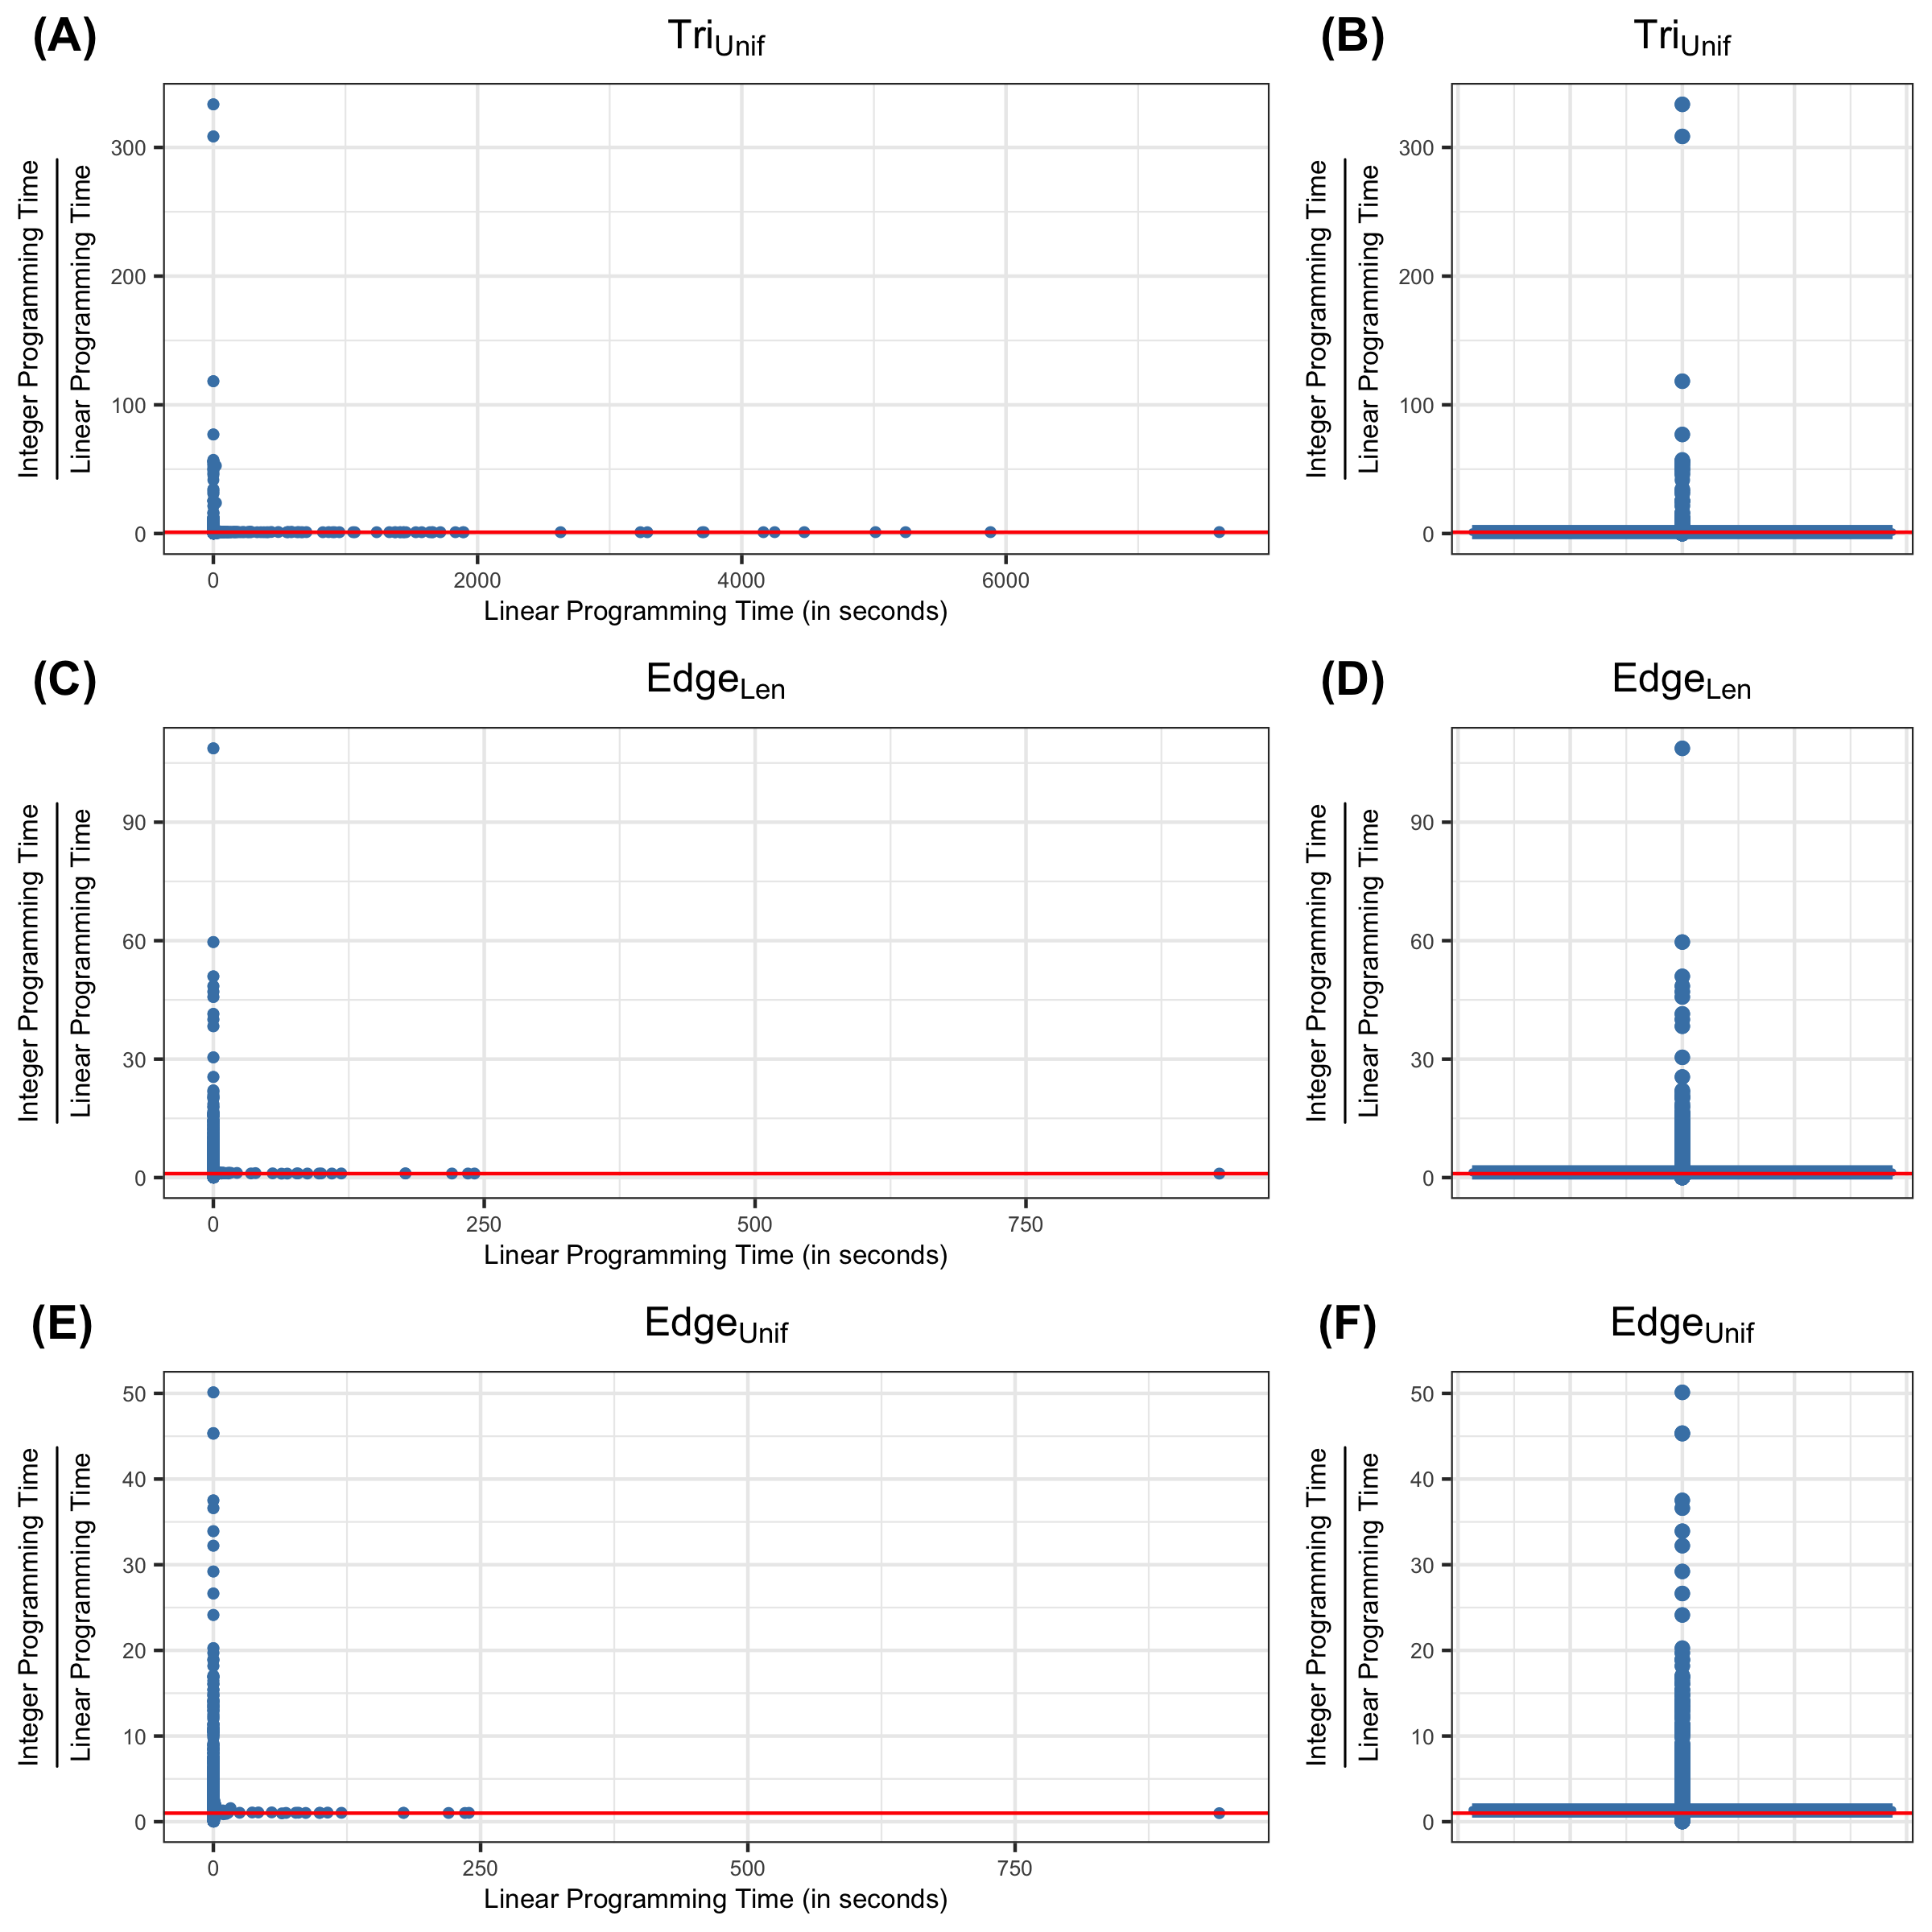
\includegraphics[width=\textwidth]{figures/IPvsLP.png}% This is a *.eps file
\end{center}
 \caption{
%  \GHP{Delete the phrase ``This figure shows the'' in every figure caption. }
 Ratio between the computation time of solving an integer programming problem Programs \ref{itm:tri_IU},\ref{itm:edge_IL}, \ref{itm:edge_IU} and the computation time of solving a linear programming problem Programs \ref{itm:tri_NIU},\ref{itm:edge_NIL}, \ref{itm:edge_NIU} for all the cycle representatives from data sets described in \se \ref{tab:realworldata} and \se \ref{tab:distributiondata}. Subfigures  \textbf{(A), (C), (E)} plot the data using scatter plots and subfigures  \textbf{(B), (D), (F)} show the same data using box plots. The vertical axis represents the ratio between the integer programming time and linear programming time of optimizing a cycle representative and the horizontal axis represents the computation time to solve the linear program. The red line in each subfigure represents the horizontal line $y=1$, where the time for each optimization is equivalent. As we can see from the box plots, the ratio between the computation time of integer programming and linear programming for most of the cycle representatives ($>50\%$) center around $1$.}\label{fig:lp_mip_ratio_df}
\end{figure}
% \begin{figure}[h!]
% \begin{center}
% 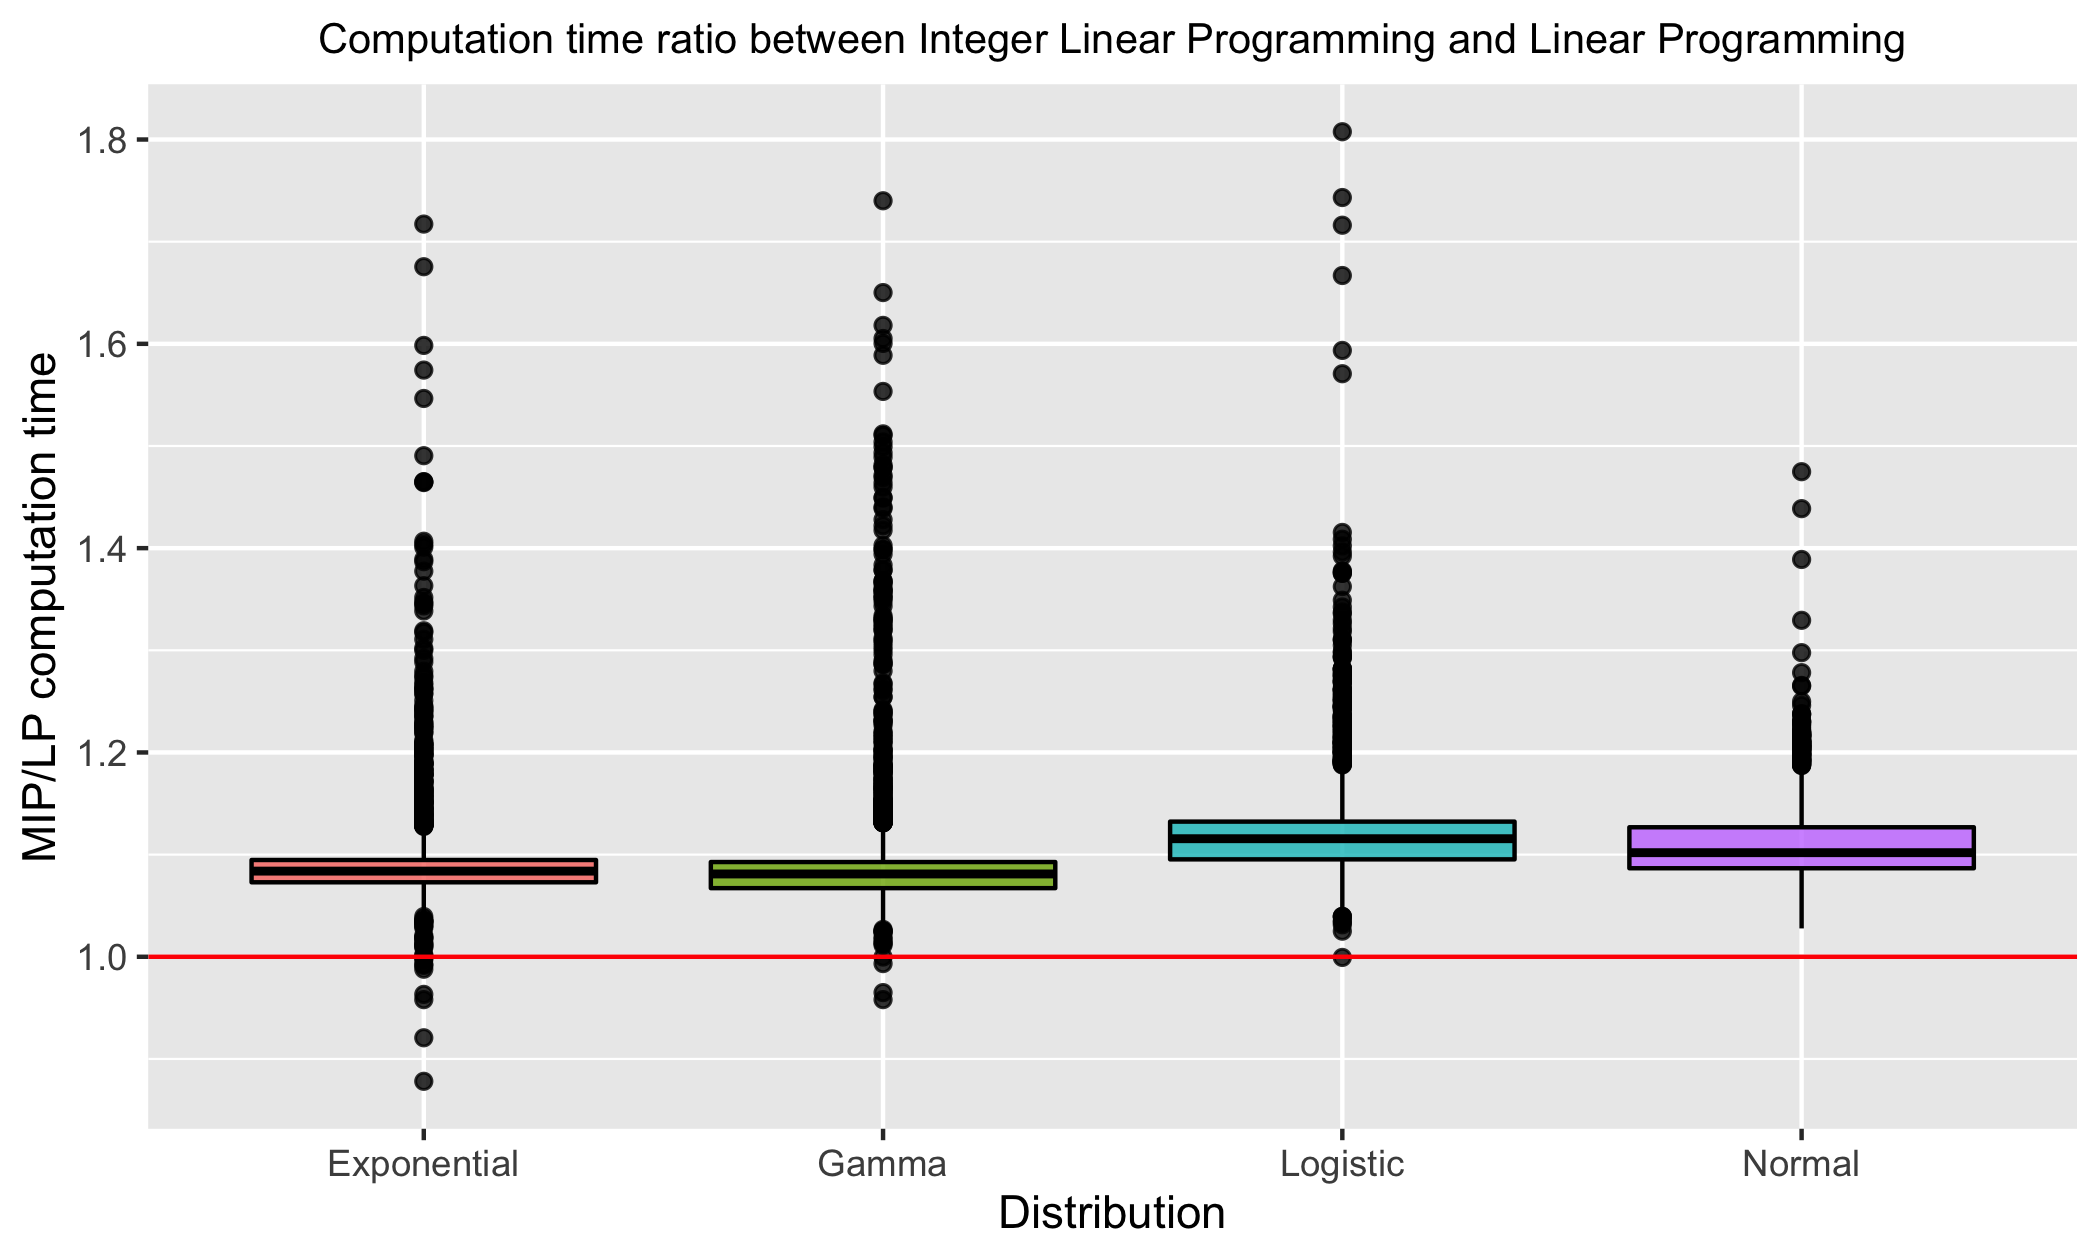
\includegraphics[width=0.8\textwidth]{figures/comptime_dist.png}% This is a *.eps file
% \end{center}
% \caption{Computation time ratio between integer programming and linear programming for randomly generated data sets. The x-axis is the distribution, and the y-axis is the ratio between the computation taken between requiring integer solutions and not requiring integer solutions. The red line marks the the value of 1. Linear programming was almost always faster than integer linear programming, although none of the displayed ratios exceed 2.0. }\label{fig:lp_mip_ratio_dist}
% \end{figure}

% delete legend 
% make x,y,title labels larger